% E90 Final Report — Howard Wang & Matthew Shiley; Advisor: Allan Moser
% Canonical project repository: https://github.com/HowardWHSrun/WALTER
% Build from this directory: pdflatex E90_Final_Report && bibtex E90_Final_Report && pdflatex E90_Final_Report && pdflatex E90_Final_Report

\documentclass[11pt]{article}
\usepackage[margin=1in]{geometry}
\usepackage[T1]{fontenc}
\usepackage[utf8]{inputenc}
\usepackage{lmodern}
\usepackage{setspace}
\usepackage{amsmath}
\usepackage{amssymb}
\usepackage{booktabs}
\usepackage{tabularx}
\usepackage{graphicx}
\usepackage{caption}
\usepackage{subcaption}
\usepackage{hyperref}
\usepackage[numbers,sort&compress]{natbib}

\hypersetup{colorlinks=true,linkcolor=blue,urlcolor=blue,citecolor=blue}
\setlength{\parskip}{0.5em}
\setlength{\parindent}{0pt}
\onehalfspacing

\newcommand{\CourseName}{Engineering 90}
\newcommand{\StudentNames}{Howard Wang and Matthew Shiley}
\newcommand{\AdvisorNames}{Allan Moser}
% Platform name: Walter (acronym W.A.L.T.E.R. = Walking Alternating Tripod for Evolutionary Research)
\newcommand{\ReportTitle}{Bio-Inspired Locomotion for \textit{Walter} (Walking Alternating Tripod for Evolutionary Research): CAD, Firmware, Optimization, and MuJoCo PPO}

\title{\ReportTitle}
\author{\StudentNames\\[0.5em]\CourseName\\Advisor(s): \AdvisorNames}
\date{\today}

\begin{document}
\maketitle

\begin{abstract}
This Engineering~90 capstone presents \emph{Walter} (\textbf{W}alking \textbf{A}lternating \textbf{T}ripod for \textbf{E}volutionary \textbf{R}esearch), a twelve-degree-of-freedom hexapod whose locomotion is organized around a \textbf{bio-inspired} alternating tripod: a low-dimensional rhythmic prior motivated by fast hexapedal gaits, realized in CAD, 3D-printed structure, hobby servos, and custom \emph{Hexapod V2} electronics including a Teensy~4.1, eighteen-channel servo driver, and BMI270 IMU. We use \textbf{classical optimization} to make that design walk: a reduced-order surrogate model and box-constrained L-BFGS-B search tune a compact open-loop sinusoidal gait, and the resulting parameters export deterministically to firmware so the physical robot runs the \textbf{same} gait law the optimizer improved.

We then use \textbf{reinforcement learning} to train more \textbf{adaptive} locomotion in simulation: Proximal Policy Optimization (PPO)~\cite{schulman2017proximal} in MuJoCo~\cite{todorov2012mujoco} with Stable-Baselines3~\cite{raffin2021stable} learns closed-loop policies that map ongoing proprioception, base kinematics, and IMU-style observations to torques, so behavior can respond to contact, balance, and task context instead of following a fixed schedule. The report summarizes surrogate metrics, exported gait parameters, a MuJoCo model view, and sample evaluations for archived policies. Full reflexive and online-adaptive firmware on the microcontroller---the natural hardware counterpart to those closed-loop observations---remains future work. Tracked purchased cost is US\$792.67 (electronics for three platforms plus three PCB orders); code and this document are at \url{https://github.com/HowardWHSrun/WALTER}.
\end{abstract}

\section{Introduction}

Reliable legged locomotion requires coordinating periodic limb motion with feedback under limited sensing and computation. Insects organize locomotor control in layers that are standard in the literature: rhythmic coordination (often modeled as CPG-like structure), fast sensory feedback, and slower parameter adjustment~\cite{aydin2023mechanosensory,chen2021adaptive}. This capstone uses that organization as bio-inspired control motivation, not as a claim that every layer is already running on the physical robot.

A recent perspective on biologically inspired machine intelligence argues that field robots and embedded agents will need to \emph{adapt} as conditions change, reuse structure across tasks, and respect tight bounds on compute, memory, and energy---capabilities grouped under lifelong learning, which remains largely open in artificial systems~\cite{kudithipudi2022biological}. Kudithipudi \emph{et al.}\ stress transfer and rapid adaptation without always returning to offline retraining, robustness when sensed data drift from training conditions, and resource-efficient learning---concerns that map directly to small hexapods that must walk on real terrain with a microcontroller-class computer. Our response is staged: we build an interpretable rhythmic substrate and optimize it with classical methods, then use reinforcement learning in simulation to learn closed-loop policies that could later be pressed toward production deployment, always keeping the biological layering story explicit.

The strongest completed work is platform and methods: a reproducible hexapod with CAD and custom PCBs; an open-loop gait optimization loop that exports parameters to firmware; and a MuJoCo PPO training and evaluation workflow with stored checkpoints and configs. A layered adaptive architecture (IMU fusion, reflexes, slow adaptation) is specified in design documents and informs observation choices in simulation, but it is not fully implemented on the MCU. The report emphasizes what was built and verified; full adaptive locomotion on the robot, and vision-augmented distance objectives, are positioned as the engineering work still required for production-style deployment, not as accomplishments of this submission.

Connecting methods to biology and to those robotics challenges~\cite{kudithipudi2022biological} proceeds as follows. The alternating tripod is a biologically motivated low-dimensional gait prior---two stance groups alternate like many fast hexapedal templates, yielding a reusable rhythmic module before any learning is applied. Surrogate optimization of a compact sinusoidal law mirrors how organisms separate pattern generation from slower corrective feedback~\cite{chen2021adaptive}: we tune that rhythm in a reduced model, then freeze it in open-loop firmware, which is lightweight enough for the embedded stack Kudithipudi \emph{et al.}\ associate with resource-constrained lifelong agents. Reinforcement learning in MuJoCo addresses adaptation and transfer in a controlled physics domain: PPO policies map proprioception, base kinematics, and IMU-style observations to torques so behavior can respond to contact and balance, partially addressing the need to handle conditions that differ from a single hand-tuned schedule (noise and domain shift between training and deployment remain central risks~\cite{kudithipudi2022biological}). IMU-based body-state cues align with how many legged systems use gravito-inertial information for posture~\cite{valenti2015quaternion,bai2019posture} and tie simulation observations to how \emph{Walter} is instrumented for eventual production transfer. RL does not by itself close the hardware adaptive loop; it prepares policies and training infrastructure that must still be validated on the robot under power, latency, and sensing limits.

The physical system is \emph{Walter}, a twelve-DOF hexapod with 3D-printed structure, servos, Teensy, driver, IMU, and \emph{Hexapod V2} PCBs (Sec.~\ref{sec:mech}--\ref{sec:elec}). Source code and this document are maintained at \url{https://github.com/HowardWHSrun/WALTER}. Sec.~\ref{sec:math-bg} states the optimization objective and the PPO machinery used in software. Sec.~\ref{sec:track1}--\ref{sec:track3} and Table~\ref{tab:tracks} summarize three tracks: (1)~surrogate optimization to firmware (completed); (2)~PPO locomotion in simulation, with IMU-capable observation modes where configured (completed as a training and evaluation stack; limited hardware deployment); (3)~vision-augmented distance objectives and tighter production integration of learned policies (remaining for deployment-scale engineering).

\section{Mathematical background: optimization and reinforcement learning}
\label{sec:math-bg}

\subsection{Reduced-order gait optimization (Track~1)}
\label{sec:math-opt}

\subsubsection{Decision variables and bounds}
The optimizer acts on a vector $\boldsymbol{\phi}\in\mathbb{R}^{25}$ matching \texttt{hexapod\_no\_imu\_optimization.py}. Indices are concatenated as
\begin{equation}
  \boldsymbol{\phi} =
  \bigl(
  \boldsymbol{\theta}_{\mathrm{abd,rest}}^{\top},
  \boldsymbol{\theta}_{\mathrm{flx,rest}}^{\top},
  \boldsymbol{\delta}_{\mathrm{abd}}^{\top},
  \boldsymbol{\delta}_{\mathrm{flx}}^{\top},
  f
  \bigr)^{\top},
\end{equation}
where each of $\boldsymbol{\theta}_{\mathrm{abd,rest}},\boldsymbol{\theta}_{\mathrm{flx,rest}},\boldsymbol{\delta}_{\mathrm{abd}},\boldsymbol{\delta}_{\mathrm{flx}}\in\mathbb{R}^{6}$ are in \emph{degrees} in the code (converted to radians internally), indexed by leg order FL, FR, ML, MR, RL, RR, and $f\in\mathbb{R}_{+}$ is the common gait frequency in hertz. Box constraints are implemented as \texttt{scipy.optimize.Bounds}: for example $f\in[0.4,\,4.0]$\,Hz; resting abduction per joint in $[-25^{\circ},25^{\circ}]$; resting flexion in $[10^{\circ},65^{\circ}]$; phase shifts in $[-120^{\circ},120^{\circ}]$. These define a feasible orthotope $\boldsymbol{\phi}_{\min}\le \boldsymbol{\phi}\le \boldsymbol{\phi}_{\max}$.

\subsubsection{Open-loop joint commands (sinusoidal law)}
Let $\omega=2\pi f$. For leg $\ell\in\{1,\ldots,6\}$ with fixed tripod offset $\psi_\ell\in\{0,\pi\}$ (alternating tripod), time $t\ge 0$, and fixed amplitude tables $\bar{a}_{\mathrm{abd},\ell}$, $\bar{a}_{\mathrm{flx},\ell}$ (defaults in code, not decision variables), the commanded abduction and flexion angles are
\begin{align}
  \phi_{\mathrm{abd},\ell}(t) &= \theta_{\mathrm{abd,rest},\ell}
    + \bar{a}_{\mathrm{abd},\ell}\,
      \sin\!\bigl(\omega t + \psi_\ell + \delta_{\mathrm{abd},\ell}\bigr), \\
  \phi_{\mathrm{flx},\ell}(t) &= \theta_{\mathrm{flx,rest},\ell}
    + \bar{a}_{\mathrm{flx},\ell}\,
      \sin\!\bigl(\omega t + \psi_\ell + \delta_{\mathrm{flx},\ell}\bigr)
    - \Delta_{\mathrm{lift},\ell}(t),
\end{align}
where $\Delta_{\mathrm{lift},\ell}$ implements swing-phase foot clearance (subtracting flexion when the abduction sine is positive), identical in structure to the firmware \texttt{LIFT\_SWING\_DEG\_PEAK} term. Velocities $\dot{\phi}_{\mathrm{abd},\ell}$, $\dot{\phi}_{\mathrm{flx},\ell}$ are obtained by differentiation and feed the planar surrogate dynamics.

\subsubsection{Surrogate planar dynamics and simulation}
The reduced model integrates an eight-dimensional state
\begin{equation}
  \mathbf{x}(t) =
  \bigl(x,\,\dot{x},\,z,\,\dot{z},\,\phi_{\mathrm{roll}},\,\dot{\phi}_{\mathrm{roll}},\,\phi_{\mathrm{pitch}},\,\dot{\phi}_{\mathrm{pitch}}\bigr)^{\top},
\end{equation}
with $\dot{\mathbf{x}}=\mathbf{f}(\mathbf{x},\boldsymbol{\phi})$ assembled from lumped masses, soft ground contact, leg thrust and support forces derived from $\phi_{\mathrm{abd},\ell}$, $\phi_{\mathrm{flx},\ell}$ and contact weights, and linear damping on body motion and attitude rates (\texttt{body\_ode} in the script). For fixed $\boldsymbol{\phi}$, the trajectory is obtained by \texttt{solve\_ivp} (Runge--Kutta) over $t\in[0,T]$ with $T$ the simulation horizon (\texttt{sim\_duration\_s}), sampled at $N$ time points (\texttt{sample\_count}).

\subsubsection{Scalar objective (explicit weighted sum)}
Let a subscript ``ss'' denote statistics evaluated on a \emph{steady-state} suffix of the horizon (the code uses the last 60\% of samples for oscillation metrics and mean speed). Write $\bar{v}_{x}$ for mean forward velocity $\mathbb{E}_{\mathrm{ss}}[\dot{x}]$, and RMS values $\mathrm{RMS}_{\mathrm{ss}}[\phi_{\mathrm{roll}}]$, $\mathrm{RMS}_{\mathrm{ss}}[\phi_{\mathrm{pitch}}]$, $\mathrm{RMS}_{\mathrm{ss}}[z]$. Let $q_{\mathrm{servo}}\ge 0$ be a slack on peak torque proxy exceeding a threshold (0.85 of stall in the implementation), and $\sigma_{\mathrm{contact}}$ the time mean of the per-timestep standard deviation of contact weights across legs. With nonnegative weights $w_{\cdot}$ matching \texttt{OptimizationConfig}, the implemented cost is
\begin{equation}
  \begin{aligned}
  \mathcal{J}(\boldsymbol{\phi}) &=
    -w_{\mathrm{fwd}}\,\bar{v}_{x}
    + w_{\mathrm{back}}\,\bigl[\max(0,-\bar{v}_{x})\bigr]^2 \\
  &\quad
    + w_{\mathrm{rp}}\Bigl(
        \mathrm{RMS}_{\mathrm{ss}}[\phi_{\mathrm{roll}}]^2
      + \mathrm{RMS}_{\mathrm{ss}}[\phi_{\mathrm{pitch}}]^2
      \Bigr)
    + w_{z}\,\mathrm{RMS}_{\mathrm{ss}}[z]^2 \\
  &\quad
    + w_{\mathrm{servo}}\,q_{\mathrm{servo}}^2
    + w_{\mathrm{contact}}\,\sigma_{\mathrm{contact}}^2
    + w_{\mathrm{reg}}\,\|\boldsymbol{\phi}-\boldsymbol{\phi}_{0}\|_{\mathrm{scaled}}^2 ,
  \end{aligned}
  \label{eq:surrogate-cost}
\end{equation}
where $\boldsymbol{\phi}_{0}$ is the default parameter vector and $\|\cdot\|_{\mathrm{scaled}}$ averages coordinatewise squared normalized deviation from the box midpoint (Tikhonov-style regularization keeping $\boldsymbol{\phi}$ in a ``reasonable'' neighborhood). Optional terms penalize shortfall below a target mean speed if \texttt{target\_forward\_speed\_mps}${}>0$. Infeasible simulations return a large penalty ($10^6$). \textbf{Design intent:} the weighted sum prioritizes forward progress while penalizing backward drift, attitude and vertical oscillation, actuator overload proxies, uneven leg loading, and deviation from nominal $\boldsymbol{\phi}_{0}$---a deliberate trade that can admit energetic gaits with visible body motion in the surrogate.

\subsubsection{Optimization algorithm and restarts}
The problem solved in software is
\begin{equation}
  \min_{\boldsymbol{\phi}}\ \mathcal{J}(\boldsymbol{\phi})
  \quad\text{subject to}\quad
  \boldsymbol{\phi}_{\min}\le \boldsymbol{\phi}\le \boldsymbol{\phi}_{\max}.
\end{equation}
\textbf{L-BFGS-B} (\texttt{scipy.optimize.minimize}, method \texttt{L-BFGS-B}) approximates curvature of $\mathcal{J}$ with a limited-memory inverse Hessian and projects each iterate onto the box. Each evaluation of $\mathcal{J}$ requires one numerical integration of the surrogate. The outer loop runs $R$ random restarts (\texttt{restarts}): one start at $\boldsymbol{\phi}_{0}$ and $R-1$ uniform samples in the box; the best $\boldsymbol{\phi}^\star$ by lowest $\mathcal{J}$ is retained. Limits \texttt{maxiter}, \texttt{maxfun}, and \texttt{ftol} cap work per restart.

The \textbf{code path} from optimization to firmware is deterministic: $\boldsymbol{\phi}^\star$ is serialized to \texttt{no\_imu\_optimization\_summary.json}; \texttt{sync\_gait\_params\_from\_json.py} emits \texttt{optimized\_gait\_params.h}; \texttt{hexapod\_openloop\_sine.ino} evaluates the same \texttt{leg\_commands()} map, applies bench degree-to-pulse gains and clamps, and streams servo targets. Thus optimization-to-code is \emph{algebraic parity}, not a learned policy.

\subsection{Policy optimization in MuJoCo (PPO with GAE)}
\label{sec:math-ppo}
Legged RL is cast as an MDP with MuJoCo supplying transitions; we use actor--critic PPO as implemented in Stable-Baselines3~\cite{raffin2021stable}. \textbf{Generalized advantage estimation} (GAE)~\cite{schulman2017proximal} builds advantages from TD residuals $\delta_t = r_t + \gamma V_\psi(s_{t+1}) - V_\psi(s_t)$:
\begin{equation}
  \hat{A}_t = \sum_{\ell=0}^{\infty}(\gamma\lambda)^\ell\,\delta_{t+\ell},
  \label{eq:gae}
\end{equation}
with $\lambda$ and discount $\gamma$ set in YAML. \textbf{PPO}~\cite{schulman2017proximal} stabilizes updates via a clipped ratio between the new and behavior policy. Define the \textbf{probability ratio}
\begin{equation}
  r_t(\theta)=\frac{\pi_\theta(a_t\mid s_t)}{\pi_{\theta_{\mathrm{old}}}(a_t\mid s_t)}.
\end{equation}
For continuous actions, $\pi_\theta$ is typically Gaussian; $r_t$ is the ratio of densities. The \textbf{clipped surrogate objective} for a batch of timesteps is
\begin{equation}
  \mathcal{L}^{\mathrm{CLIP}}(\theta)
  = \mathbb{E}_t\Bigl[
 \min\bigl(
      r_t(\theta)\,\hat{A}_t,\;
      \mathrm{clip}\bigl(r_t(\theta),1-\epsilon,1+\epsilon\bigr)\,\hat{A}_t
    \bigr)
  \Bigr],
  \label{eq:ppo-clip}
\end{equation}
with clip range $\epsilon\in(0,1)$ (often $0.2$). Large policy steps that inflate $r_t$ when $\hat{A}_t>0$ (or shrink $r_t$ when $\hat{A}_t<0$) are clipped so the effective objective stops increasing, reducing catastrophic updates common in vanilla policy gradients.

Let $\hat{R}_t$ denote a target return for the critic (e.g., $n$-step return or GAE-backed value target). With coefficients $c_v,c_e>0$, the \textbf{composite loss} maximized in practice is the negative of
\begin{equation}
  \mathcal{L}_{\mathrm{total}}(\theta,\psi)
  = -\mathcal{L}^{\mathrm{CLIP}}(\theta)
  + c_v\,\mathbb{E}_t\bigl[(V_\psi(s_t)-\hat{R}_t)^2\bigr]
  - c_e\,\mathbb{E}_t\bigl[H(\pi_\theta(\cdot\mid s_t))\bigr],
  \label{eq:ppo-total-loss}
\end{equation}
where $H$ is differential entropy for Gaussian policies. Minimizing $\mathcal{L}_{\mathrm{total}}$ corresponds to ascending $\mathcal{L}^{\mathrm{CLIP}}$ while fitting the critic and discouraging collapse of exploratory variance. Updates use minibatches over several epochs on each rollout buffer; hyperparameters (learning rate, rollout length \texttt{n\_steps}, batch size, $\gamma$, $\lambda$, $\epsilon$, $c_v$, $c_e$) are set in YAML under \texttt{hexapod\_training\_new/configs/}.

\section{Track I: Surrogate optimization and firmware export}
\label{sec:track1}

This track \textbf{implements} Sec.~\ref{sec:math-opt}: the $\boldsymbol{\phi}$ parameterization, sinusoidal \texttt{leg\_commands()}, the eight-state surrogate, cost~\eqref{eq:surrogate-cost}, box-constrained L-BFGS-B with restarts, and a \textbf{deterministic path} from $\boldsymbol{\phi}^\star$ to C headers and \texttt{hexapod\_openloop\_sine}. The workflow isolates a tunable open-loop rhythm before IMU-closed-loop layers are required.

\textbf{What we shipped.} Optimizer script, summary JSON, JSON-to-header sync, and open-loop Arduino sketch with exported gains. Quantitative surrogate outputs appear in Tables~\ref{tab:sim}--\ref{tab:opt-params}; the high-fidelity MuJoCo asset used for RL appears in Fig.~\ref{fig:mujoco}.

\section{Track II: PPO locomotion in MuJoCo}
\label{sec:track2}

The policy $\pi_\theta(a|s)$ conditions on \textbf{proprioception} (joint positions and velocities), simulator \textbf{base kinematics}, and---in IMU-focused YAML configs---\textbf{accelerometer and gyroscope} channels (or complementary-filter-style stacks) so roll, pitch, and body rates align with how \emph{Walter} is sensed on hardware. \textbf{Tripod structure} enters through phase features, structured policy heads (e.g., sCPG variants), or reward shaping, depending on the experiment. Training uses Eqs.~\eqref{eq:gae}--\eqref{eq:ppo-clip} on MuJoCo rollouts.

\textbf{Scope.} The team \textbf{built, trained, and evaluated} policies in simulation, archived checkpoints, and wrote short evaluation summaries for representative runs (Table~\ref{tab:rl-eval}). Deploying a trained policy as the primary closed-loop driver on the physical robot---with the same observation latency and actuation path as firmware---was \textbf{out of scope} for verification in this report.

\section{Track III: Vision, distance-centric rewards, and production path}
\label{sec:track3}

For production deployment, the observation should eventually fuse proprioception and IMU with visual odometry or pose from an overhead or onboard camera so rewards can emphasize distance traveled with less simulator-privileged state. Let $p_t\in\mathbb{R}^2$ be horizontal pose from visual integration or fiducials, and consider forward displacement $x_t-x_0$. A natural reward increment is
\begin{equation}
  r_t = \alpha\,(x_{t+1}-x_t) - \beta\,\|\omega_t\|^2 - \rho\,\mathrm{penalty}_{\mathrm{fall}} - \kappa\,\mathrm{TV}(a)_t,
\end{equation}
with IMU rates $\omega_t$ penalizing harsh attitude changes, and optional terms for staying upright. The observation becomes $s_t=[s_t^{\mathrm{IMU/proprio}},\, f_t]$ where $f_t$ carries visual features or estimated pose; PPO then uses the same surrogate~\eqref{eq:ppo-clip} with expanded input dimension. Bringing this stack to production requires closing sim-to-real on vision and latency, defining rewards from estimated versus ground-truth motion, and preserving the tripod prior while learning residuals---the same adaptation and robustness pressures highlighted for embedded lifelong systems~\cite{kudithipudi2022biological}.

\begin{table}[htbp]
  \centering
  \caption{Summary of the three development tracks for \emph{Walter}.}
  \label{tab:tracks}
  \begin{tabular}{@{}p{0.14\linewidth}p{0.46\linewidth}p{0.32\linewidth}@{}}
    \toprule
    Track & Technical core & Outcome in this capstone \\
    \midrule
    I & Surrogate $\mathcal{J}(\boldsymbol{\phi})$ \eqref{eq:surrogate-cost}; L-BFGS-B; JSON$\to$\texttt{.h}$\to$ open-loop firmware & \textbf{Completed:} optimization exported and flashed path demonstrated \\
    II & PPO \eqref{eq:ppo-clip}; GAE \eqref{eq:gae}; MuJoCo env; IMU modes in config & \textbf{Completed:} training/eval pipeline and archived runs; hardware policy deployment not fully exercised here \\
    III & Visual or pose features $f_t$; distance-centric rewards & Remaining for production: not implemented in repo; spec and math only \\
    \bottomrule
  \end{tabular}
\end{table}

\section{Technical Discussion}

\subsection{Biological and control context}
Decentralized feedback atop rhythmic coordination remains a standard idiom for insect locomotion~\cite{aydin2023mechanosensory,chen2021adaptive}. Attitude filters for accelerometer--gyro fusion~\cite{valenti2015quaternion,zhang2021attitude} and posture control on terrain~\cite{bai2019posture} inform the IMU observation choices in simulation. Disturbance-triggered transitions~\cite{johnson2010disturbance} motivate reflex layers in the design spec, not a completed hardware demo in this capstone.

\subsection{Planned adaptive layer (design specification)}
Internal architecture notes (\texttt{docs/ARCHITECTURE.md}) describe a \textbf{future} two-timescale stack: a \textbf{fast tick} ($\sim$10--20\,ms) for IMU read, attitude fusion, stability score $S$, reflex adjustments, gait interpolation, and servo commands; and a \textbf{slow tick} (per gait cycle) for windowed costs and optional parameter adaptation. That design informed IMU-inclusive observation modes in simulation; it is \textbf{not} claimed as deployed firmware here. The complementary blend
\begin{equation}
\alpha \in (0,1),\quad
\theta_{\mathrm{roll}} \leftarrow \alpha(\theta_{\mathrm{roll}} + \omega_x \Delta t) + (1-\alpha)\,\theta_{\mathrm{roll,accel}},
\end{equation}
(and analogously for pitch) is the nominal attitude update.

\subsection{Open-loop sinusoidal gait (implemented)}
For the no-IMU milestone, each leg follows resting abduction and flexion angles plus sinusoidal variation at common frequency $f$, with tripod group~B offset by $\pi$ from group~A. This is the same law optimized in Sec.~\ref{sec:math-opt} and delivered in Track~I (Sec.~\ref{sec:track1}). Amplitudes follow default tables shared by Python and \texttt{optimized\_gait\_params.h}.

\subsection{MuJoCo and reinforcement learning (simulation)}
High-fidelity training uses Gymnasium + MuJoCo~\cite{todorov2012mujoco} with PPO~\cite{schulman2017proximal} as implemented in Stable-Baselines3~\cite{raffin2021stable}; the mathematical objective is Eq.~\eqref{eq:ppo-clip} with advantages~\eqref{eq:gae}. Tracks~II--III (Sec.~\ref{sec:track2}--\ref{sec:track3}) specialize the observation and reward; YAML configs set $\gamma$, $\lambda$, learning rate, network widths, PD gains, and terrain. A representative static render of the simulation model appears in Fig.~\ref{fig:mujoco} (Sec.~\ref{sec:res-mujoco}).

\subsection{Mechanical design: CAD and 3D-printed parts}
\label{sec:mech}
Walter's chassis and legs are built from \textbf{parts designed in CAD} and produced by \textbf{additive manufacturing} (3D printing): a central body, six leg assemblies, and two-degree-of-freedom linkages per leg (abduction and flexion axes) that mate to the servo output splines. The design prioritizes a repeatable assembly for twelve actuated joints, clearance for wiring, and attachment of the electronics tray and battery. Figure~\ref{fig:walter} shows an overall render; Figure~\ref{fig:walter-parts} shows the body, leg, and linkage components used in the assembly. Fasteners and servo hardware complete the mechanical stack; material usage (filament mass) and printed-part cost are not included in the dollar totals in Tables~\ref{tab:cost}--\ref{tab:grand}.

\begin{figure}[htbp]
  \centering
  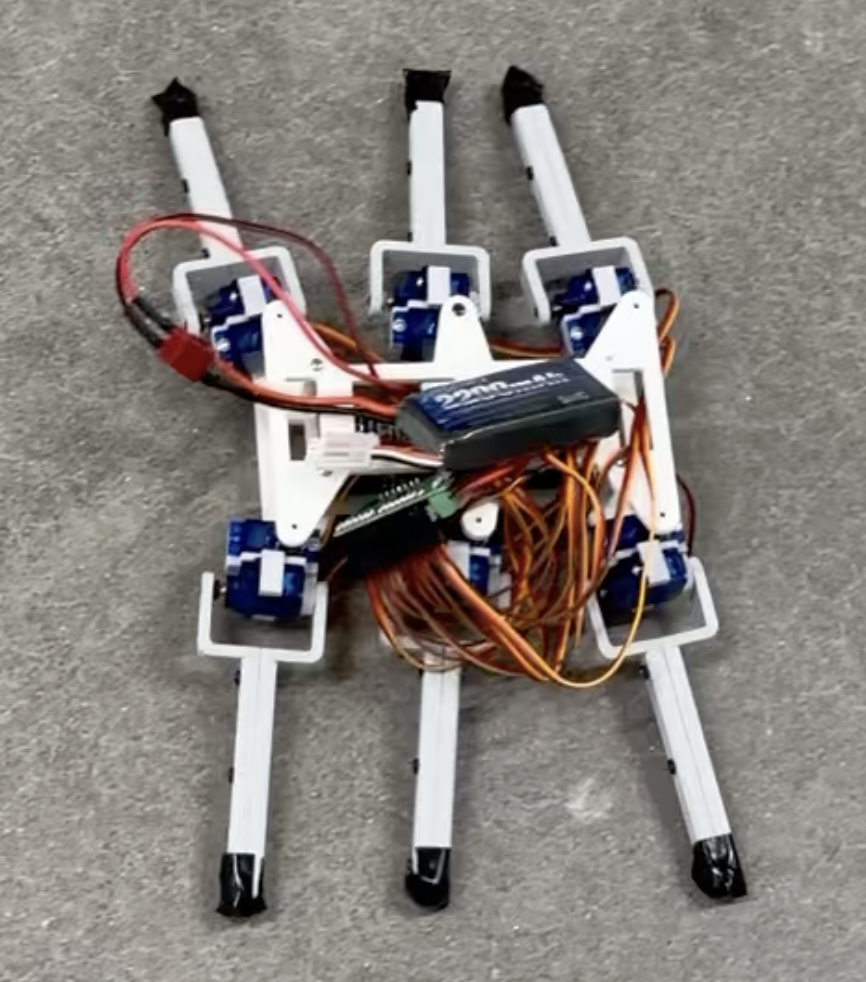
\includegraphics[width=0.92\linewidth]{walter_assembly.png}
  \caption{Walter: full-assembly render of the twelve-DOF hexapod (CAD; Walking Alternating Tripod for Evolutionary Research).}
  \label{fig:walter}
\end{figure}

\begin{figure}[htbp]
  \centering
  \begin{subfigure}[b]{0.32\linewidth}
    \centering
    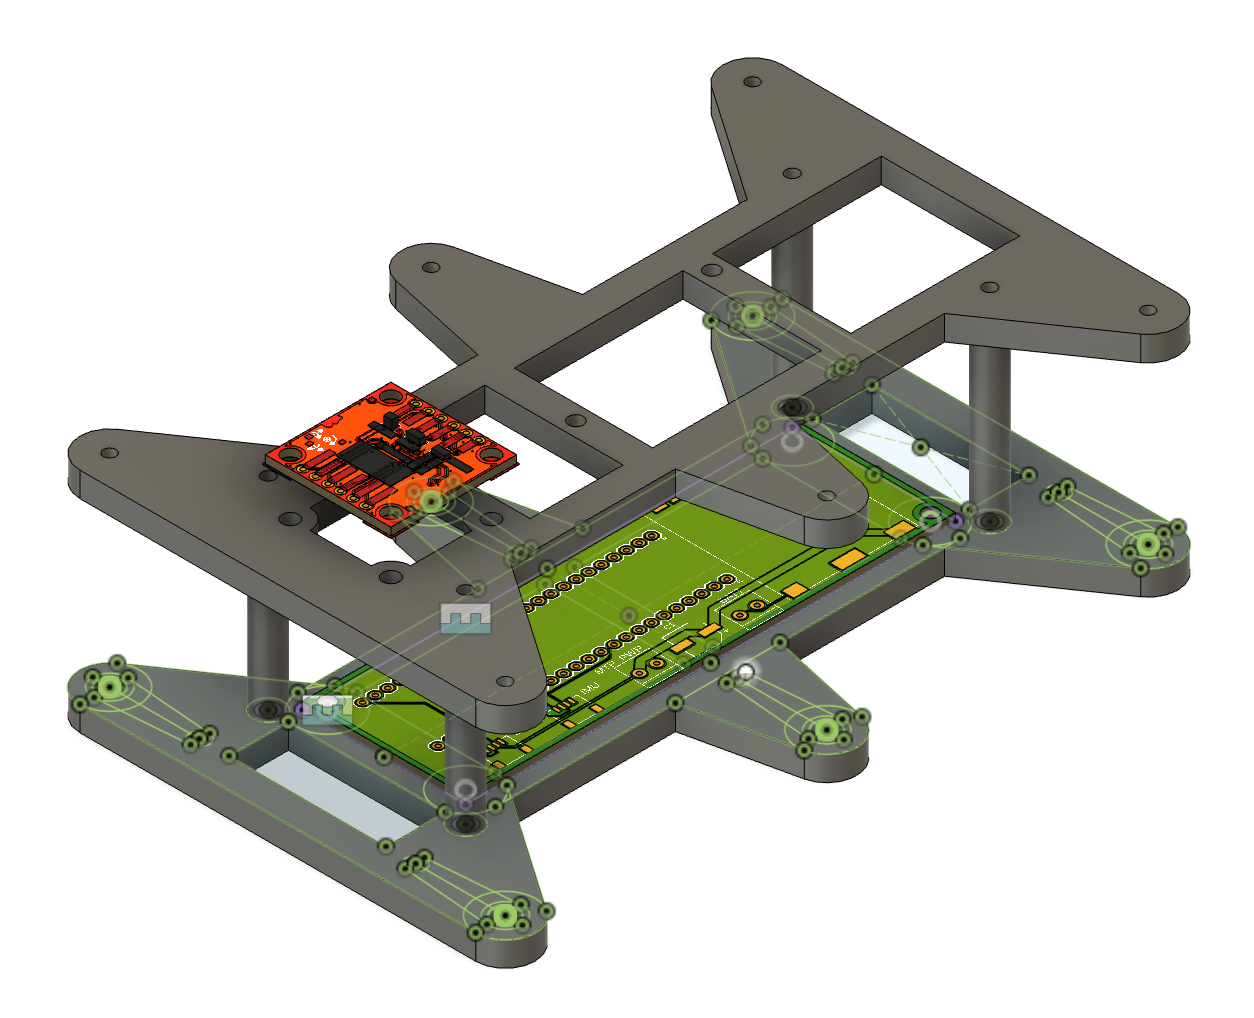
\includegraphics[width=\linewidth]{Body.png}
    \caption{Body}
  \end{subfigure}\hfill
  \begin{subfigure}[b]{0.32\linewidth}
    \centering
    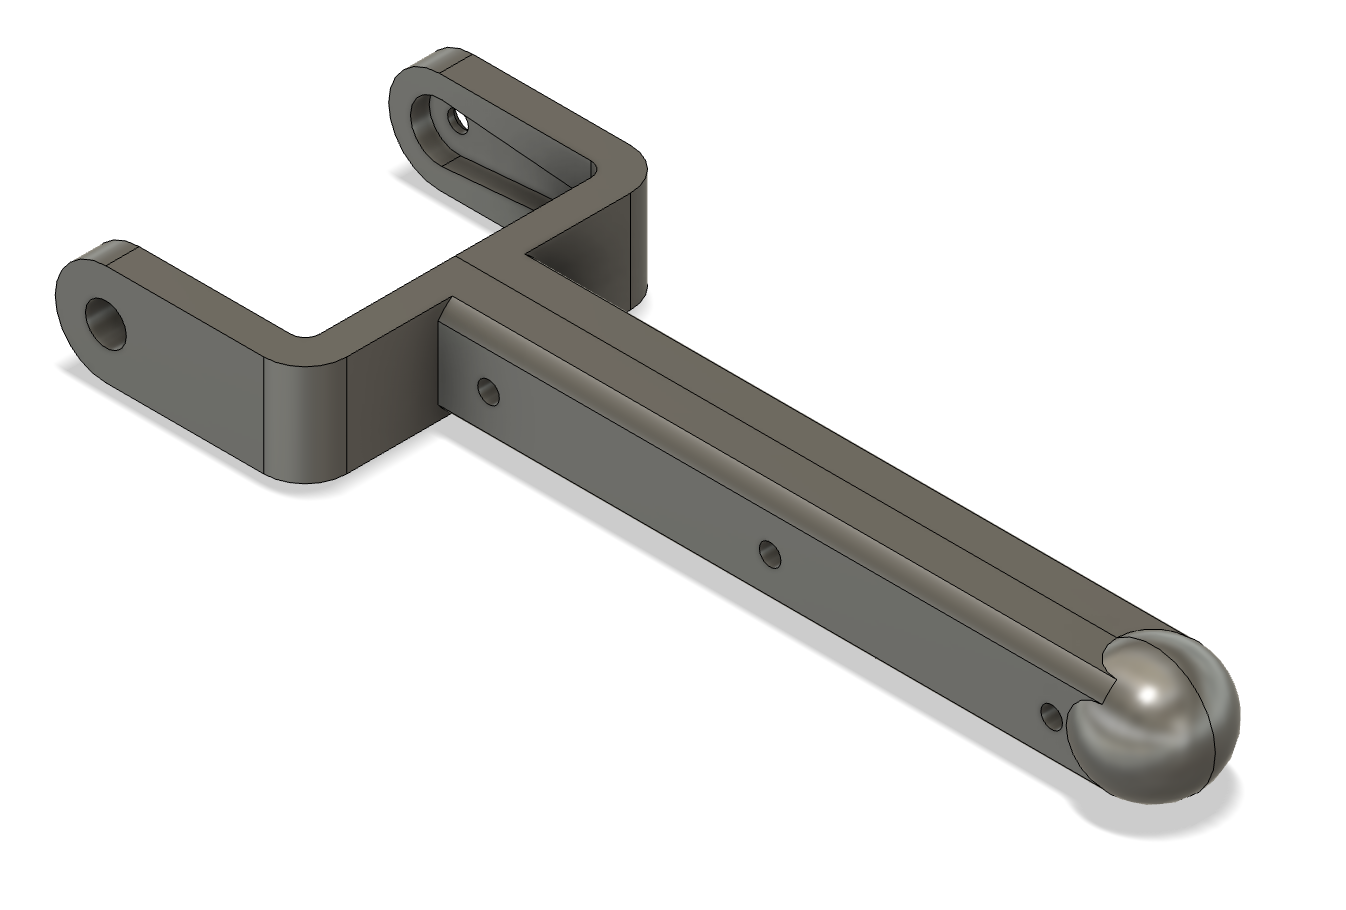
\includegraphics[width=\linewidth]{Legs.png}
    \caption{Leg assemblies}
  \end{subfigure}\hfill
  \begin{subfigure}[b]{0.32\linewidth}
    \centering
    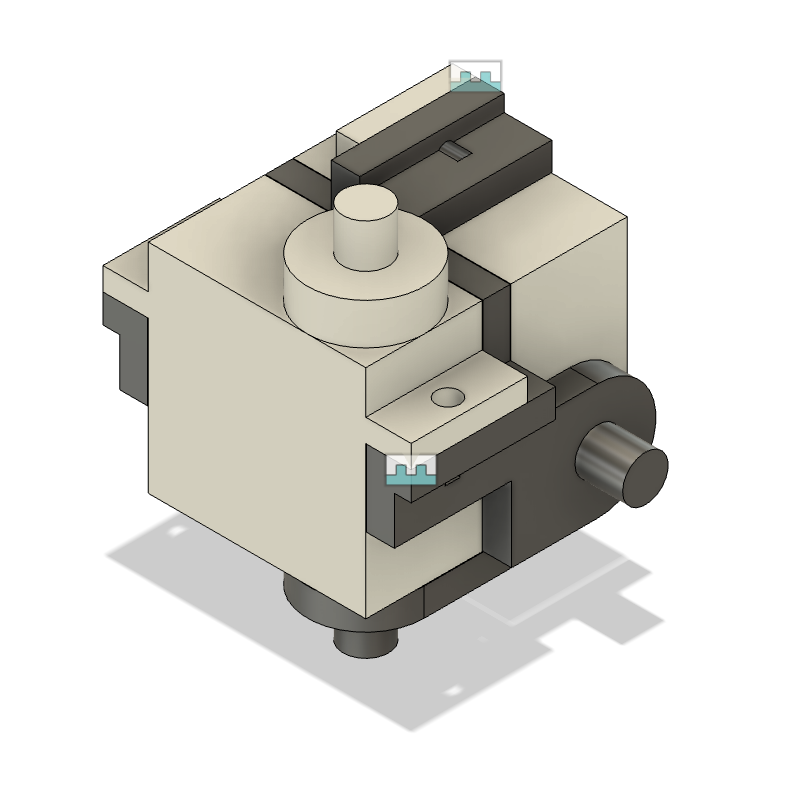
\includegraphics[width=\linewidth]{Linkage.png}
    \caption{Linkage}
  \end{subfigure}
  \caption{CAD-designed 3D-printed subassemblies for Walter: chassis, legs, and per-leg linkage.}
  \label{fig:walter-parts}
\end{figure}

\subsection{Electronics, Hexapod V2 PCB, and safety}
\label{sec:elec}
The bill of materials matches purchased components: Teensy-class MCU (SparkFun 16771), Pololu 1354 eighteen-channel driver, buck converter, BMI270 via Qwiic cabling, dual-cell LiPo and charger, terminals, and servos. Custom \emph{Hexapod V2} PCBs (revision v5 dated 2026-04-03 on the latest order) integrate power and signal routing for Walter's stack; Figure~\ref{fig:pcb} shows a board photo and schematic excerpt. \texttt{docs/FIRMWARE.md} records UART to the servo controller, channel ordering FL/FR/ML/MR/RL/RR with abduction then flexion per leg, and pulse mapping $u_k = \mathrm{clamp}(c_k + d_k q_k)$ (typical bounds 600--2400\,$\mu$s). Open-loop firmware applies degree-to-command gains and clamps before streaming compact-protocol targets; these bench gains are not outputs of the reduced-order optimizer.

\begin{figure}[htbp]
  \centering
  \begin{subfigure}[b]{0.48\linewidth}
    \centering
    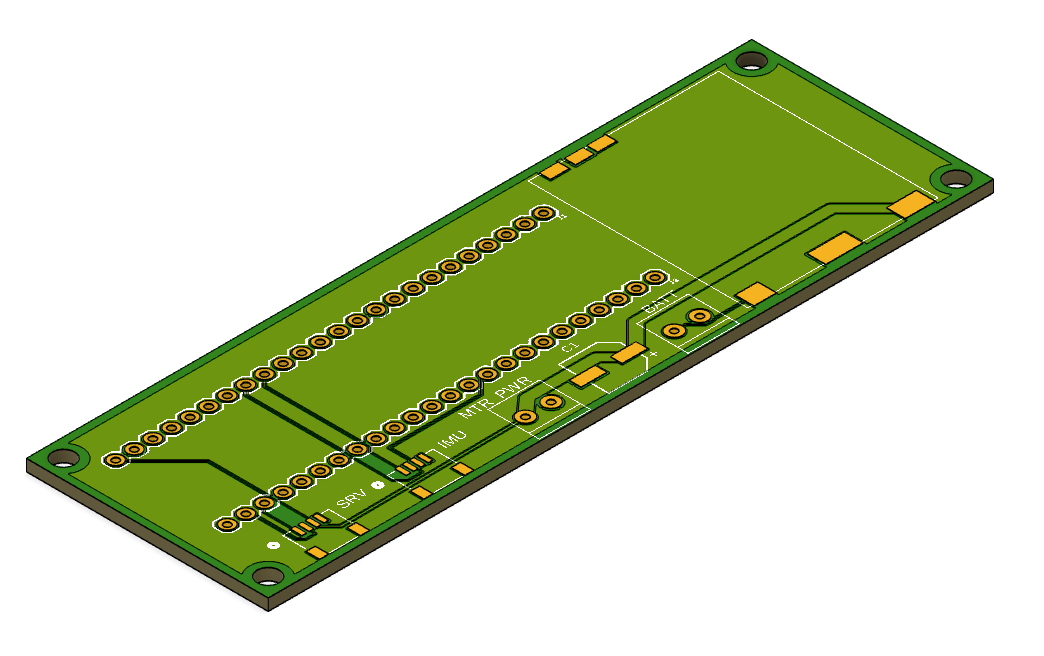
\includegraphics[width=\linewidth]{pcb_board.png}
    \caption{Assembled PCB (Hexapod V2)}
  \end{subfigure}\hfill
  \begin{subfigure}[b]{0.48\linewidth}
    \centering
    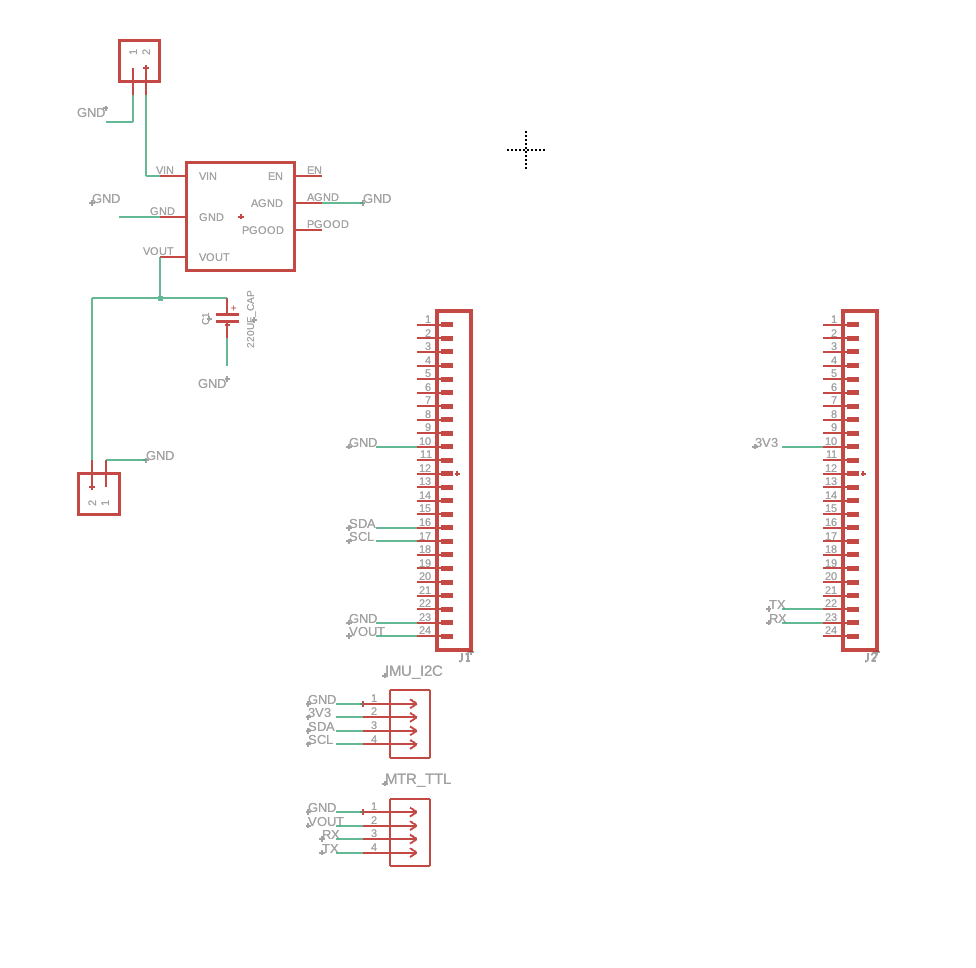
\includegraphics[width=\linewidth]{pcb_schematic.png}
    \caption{Schematic (excerpt)}
  \end{subfigure}
  \caption{Custom electronics for Walter: Hexapod V2 board and schematic.}
  \label{fig:pcb}
\end{figure}

\section{Requirements and Constraints}

\subsection{Source of requirements}
Engineering requirements are traced to phase exit criteria in \texttt{docs/PHASES.md} (Phases~1--4: IMU telemetry, reflexes, cautious mode and recovery, online adaptation), supplemented by safety and interface constraints in \texttt{docs/FIRMWARE.md} and the open-loop scope in \texttt{firmware/hexapod\_openloop\_sine/README.md}. \texttt{PHASES.md} serves as the team's consolidated requirements-and-constraints specification for firmware behavior.

\subsection{Summary: met vs.\ not met}
\textbf{Satisfied in this project:} discrete tripod baseline firmware; open-loop optimization with JSON export and header sync; calibration sketches; CAD-documented mechanical design (Figs.~\ref{fig:walter}--\ref{fig:walter-parts}); a MuJoCo PPO workflow with configs, training scripts, checkpoints, and evaluation writeups. \textbf{Not satisfied against the internal phased firmware spec:} Phases~1--4 adaptive behaviors (telemetry-only through online adaptation) are largely \textbf{not implemented} on the MCU in the snapshot summarized below.

\begin{table}[htbp]
  \centering
  \caption{Requirement traceability (internal \texttt{PHASES.md} vs.\ delivered work).}
  \label{tab:req}
  \begin{tabular}{@{}p{0.06\linewidth}p{0.36\linewidth}p{0.12\linewidth}p{0.38\linewidth}@{}}
    \toprule
    ID & Requirement & Status & Evidence / notes \\
    \midrule
    R1 & Phase~1: IMU read, complementary filter, USB telemetry $\sim$50\,Hz; gait unchanged & Not met (in repo) & \texttt{PHASES.md}; folder may be missing \\
    R2 & Phase~2: postural reflexes, clamps, serial tuning, EEPROM & Not met (in repo) & \texttt{ARCHITECTURE.md} pseudocode \\
    R3 & Phase~3: stability score, cautious mode, push recovery, fall freeze & Not met (in repo) & Documented only \\
    R4 & Phase~4: five-parameter adaptation, cost $J$, SPSA/bandit, EEPROM & Not met (in repo) & Documented only \\
    R5 & Hardware: MCU + eighteen-channel driver + servos + documented map + PCBs + Walter mechanical CAD/3D parts & Met & BOM, Figs.~\ref{fig:walter}--\ref{fig:pcb}, \texttt{FIRMWARE.md} \\
    R6 & Safety: pulse clamps; parameter slew (adaptive layer) & Partial & Clamps in v2/openloop; slew in spec \\
    R7 & Open-loop: optimizer/firmware parity; JSON export & Met & Optimizer, \texttt{sync\_gait\_params\_from\_json.py} \\
    R8 & Simulation: MuJoCo env, PPO training, documented evals & Met & \texttt{hexapod\_training\_new/}, \texttt{e90\_repo/released\_checkpoints/} \\
    \bottomrule
  \end{tabular}
\end{table}

\subsection{Project cost}
Tables~\ref{tab:cost}--\ref{tab:pcb} summarize \textbf{purchased} electronics (three identical platforms) and \textbf{fabrication} costs for three PCB/stencil orders. Table~\ref{tab:grand} states the \textbf{grand total} for those categories only; filament, fasteners, and shop labor are outside the accounting. Servo counts in Table~\ref{tab:cost} are per platform (eight units listed per BOM line); completing twelve DOF per robot may require additional servos beyond those lines if not already stocked.

\begin{table}[htbp]
  \centering
  \caption{Electronics bill of materials, \textbf{one platform} (USD). The team purchased three identical sets.}
  \label{tab:cost}
  \footnotesize
  \setlength{\tabcolsep}{4pt}
  \begin{tabular}{@{}p{2.35cm}p{4.35cm}p{1.15cm}rrr@{}}
    \toprule
    Part & Description & Vendor & Qty & Unit & Line \\
    \midrule
    SparkFun 16771 & Microcontroller & DigiKey & 1 & 37.20 & 37.20 \\
    Pololu 1354 & 18-channel servo driver & DigiKey & 1 & 46.95 & 46.95 \\
    DFRobot DFR1202 & Step-down buck converter & DFRobot & 1 & 12.90 & 12.90 \\
    SparkFun BMI270 & 6-DoF IMU & DigiKey & 1 & 18.50 & 18.50 \\
    SparkFun 11855 & 2$\times$7.4\,V LiPo + charger & Amazon & 1 & 27.99 & 27.99 \\
    SparkFun 14417 & Female Qwiic connector & DigiKey & 2 & 0.60 & 1.20 \\
    SparkFun 17259 & 100\,mm Qwiic cable & DigiKey & 1 & 1.95 & 1.95 \\
    SparkFun 17261 & Qwiic cable to female header & DigiKey & 1 & 1.95 & 1.95 \\
    Amphenol YO0201500000G & 1$\times$2 screw-down terminal & DigiKey & 2 & 1.28 & 2.56 \\
    DFRobot SER0039 & Servo motor & DigiKey & 8 & 5.90 & 47.20 \\
    \midrule
    \textbf{Subtotal} & \textbf{one platform} & & & & \textbf{198.40} \\
    \textbf{Electronics total} & \textbf{three platforms ($\times$3)} & & & & \textbf{595.20} \\
    \bottomrule
  \end{tabular}
\end{table}
\normalsize

\begin{table}[htbp]
  \centering
  \caption{PCB and stencil orders, \emph{Hexapod V2} (USD order totals including merchandise, shipping, duties/taxes, and sales tax where charged by the vendor).}
  \label{tab:pcb}
  \footnotesize
  \begin{tabular}{@{}p{3.1cm}p{4.6cm}p{2.0cm}r@{}}
    \toprule
    Order ID & Description / notes & Status & Total \\
    \midrule
    Y4-11911448A & PCB prototype (5\,pcs) + SMT stencil; v5\_2026-04-03 & Awaiting payment & 74.24 \\
    W2026030804205410 & PCB + stencil shipment & Shipped & 68.26 \\
    W2026021709554129 & PCB + stencil (earlier order) & Shipped & 54.97 \\
    \midrule
    \textbf{PCB subtotal} & & & \textbf{197.47} \\
    \bottomrule
  \end{tabular}
\end{table}
\normalsize

\begin{table}[htbp]
  \centering
  \caption{Grand total project cost (USD) for reported purchases and fabrication.}
  \label{tab:grand}
  \begin{tabular}{@{}lr@{}}
    \toprule
    Category & Amount \\
    \midrule
    Electronics (three platforms) & 595.20 \\
    PCB fabrication and stencils (three orders) & 197.47 \\
    \midrule
    \textbf{Grand total} & \textbf{792.67} \\
    \bottomrule
  \end{tabular}
\end{table}

\section{Methods}

\subsection{Mechanical assembly (\emph{Walter})}
Printed body and leg components are fastened per the CAD design; each leg receives two servos driving abduction and flexion through the linkage. The custom PCB mounts to the chassis and connects to the Pololu driver and Teensy; power and ground respect the buck converter and screw terminals from the BOM. Bench alignment uses \texttt{set\_zero} and side-only test sketches before closed-loop or open-loop gait tests.

\subsection{Baseline discrete gait}
\texttt{firmware/hexapod\_walking\_v2/hexapod\_walking\_v2.ino} implements a deterministic tripod state machine with smoothed keyframes (\texttt{moveSmoothTo}).

\subsection{Reduced-order simulation optimization}
\texttt{hexapod\_brain\_roadmap copy/ode\_optimization\_no\_imu/hexapod\_no\_imu\_optimization.py} integrates the surrogate model with \texttt{scipy.integrate.solve\_ivp}, evaluates the objective on a steady-state window, and calls \texttt{scipy.optimize.minimize} (L-BFGS-B). Outputs include \texttt{no\_imu\_optimization\_summary.json} and optional CSV/plots.

\subsection{Parameter sync and open-loop firmware}
From \texttt{firmware/hexapod\_openloop\_sine/}, run \texttt{python3 sync\_gait\_params\_from\_json.py} to regenerate \texttt{optimized\_gait\_params.h}. The sketch evaluates the sinusoidal law at \texttt{INTERP\_DELAY\_MS} (default 10\,ms), applies startup frequency ramping, maps degrees to integer commands, clamps, and sends Pololu compact-protocol targets on \texttt{Serial1}.

\subsection{Bench testing and calibration}
\texttt{firmware/set\_zero/} and side-only test sketches support calibration. The open-loop README documents sign and scale tuning when feet drag or the robot shuffles backward.

\subsection{MuJoCo PPO training and evaluation}
The project produced a \textbf{reusable training workflow}: \texttt{train.py} reads YAML from \texttt{configs/}, writes summaries, checkpoints, and logs under \texttt{runs/<run\_name>/}, and pairs with \texttt{evaluate.py} using the same configuration. Released material includes zipped policies, per-run evaluation folders with \texttt{REPORT.md} summaries, and metadata for reproducibility and reporting.

\section{Results}
\label{sec:results}

\subsection{Reduced-order optimization (surrogate model)}
Table~\ref{tab:sim} summarizes \texttt{hexapod\_brain\_roadmap copy/ode\_optimization\_no\_imu/no\_imu\_optimization\_summary.json}. These numbers describe the \emph{planar surrogate} only; they are not a guarantee of on-robot speed or stability.

\begin{table}[htbp]
  \centering
  \caption{Optimizer-reported metrics (committed summary JSON).}
  \label{tab:sim}
  \begin{tabular}{@{}lr@{}}
    \toprule
    Quantity & Value \\
    \midrule
    Gait frequency $f$ & 1.80\,Hz \\
    Mean forward speed (steady window) & 0.234\,m/s \\
    Total displacement (rollout) & 1.86\,m \\
    Roll RMS & 0.440\,rad \\
    Pitch RMS & $\sim 0$ (near zero in file) \\
    Vertical position RMS & 0.086\,m \\
    Peak servo usage ratio (proxy) & 0.152 \\
    Contact balance std.\ dev. & 0.388 \\
    Dominant oscillation frequency (estimated) & 3.54\,Hz \\
    Objective cost $\mathcal{J}(\boldsymbol{\phi}^\star)$ & $-228.38$ \\
    \bottomrule
  \end{tabular}
\end{table}

\textbf{Reading Table~\ref{tab:sim}.} Mean forward speed $\approx 0.23$\,m/s and $\approx 1.9$\,m travel over the surrogate horizon indicate the optimizer found a gait that moves the reduced model forward. Roll RMS near $0.44$\,rad is \textbf{large}: the surrogate tolerates body oscillation in exchange for speed under the chosen weights. Pitch RMS near zero reflects the planar symmetry of the lumped model more than a claim of perfect hardware pitch stability. Peak servo usage and contact-balance spread show the solution stays inside soft actuator and support proxies, but \textbf{contact and torque models are coarse}---hardware will differ once pulses, friction, and foot slip are included.

Table~\ref{tab:opt-params} lists $\boldsymbol{\phi}^\star$ exported to \texttt{optimized\_gait\_params.h}. Flexion phase shifts sit at the lower bound ($-90^\circ$): the optimizer traded stride phasing aggressively for the surrogate objective; bench tuning may move off that bound. Rest angles cluster in physically plausible ranges; frequency near $1.8$\,Hz matches a moderate stride rate for small hexapods in simulation-like settings.

\begin{table}[htbp]
  \centering
  \caption{Optimized decision variables $\boldsymbol{\phi}^\star$ from L-BFGS-B (same JSON as Table~\ref{tab:sim}). Angles in degrees; leg order FL, FR, ML, MR, RL, RR.}
  \label{tab:opt-params}
  \footnotesize
  \setlength{\tabcolsep}{6pt}
  \begin{tabular}{@{}p{3.5cm}p{9.2cm}@{}}
    \toprule
    Quantity & Value \\
    \midrule
    Gait frequency $f$ & 1.800\,Hz \\
    Abduction rest $\boldsymbol{\theta}_{\mathrm{abd,rest}}$ & $(10,\,10,\,0,\,0,\,-10,\,-10)$ \\
    Flexion rest $\boldsymbol{\theta}_{\mathrm{flx,rest}}$ & $(32.00,\,32.00,\,34.00,\,34.00,\,32.00,\,32.00)$ \\
    Abduction phase $\boldsymbol{\delta}_{\mathrm{abd}}$ & $\approx \mathbf{0}$ (magnitude $<10^{-6}$\,deg) \\
    Flexion phase $\boldsymbol{\delta}_{\mathrm{flx}}$ & $(-90,\,-90,\,-90,\,-90,\,-90,\,-90)$ \\
    Swing lift amplitude & 12.0\,deg (\texttt{lift\_swing\_deg\_peak}) \\
    \bottomrule
  \end{tabular}
\end{table}
\normalsize

\subsection{MuJoCo simulation (high-fidelity model)}
\label{sec:res-mujoco}
Track~II--III training uses Gymnasium with the MuJoCo asset \texttt{hexapod\_training\_new/assets/hexapod.xml}: checkerboard ground, twelve torque-controlled joints, and RK4 integration at 0.002\,s (see configs for frame skipping). Figure~\ref{fig:mujoco} is an \textbf{offscreen MuJoCo render} (software \texttt{Renderer}, no interactive viewer): the model was advanced under gravity with zero actuator commands until the body settled on the plane, then a fixed camera was used. The view documents the mesh, materials, and lighting used for PPO rollouts; it is not a policy-controlled frame. Interactive inspection is available via \texttt{scripts/live\_mujoco\_viewer.py} with a trained checkpoint.

\begin{figure}[htbp]
  \centering
  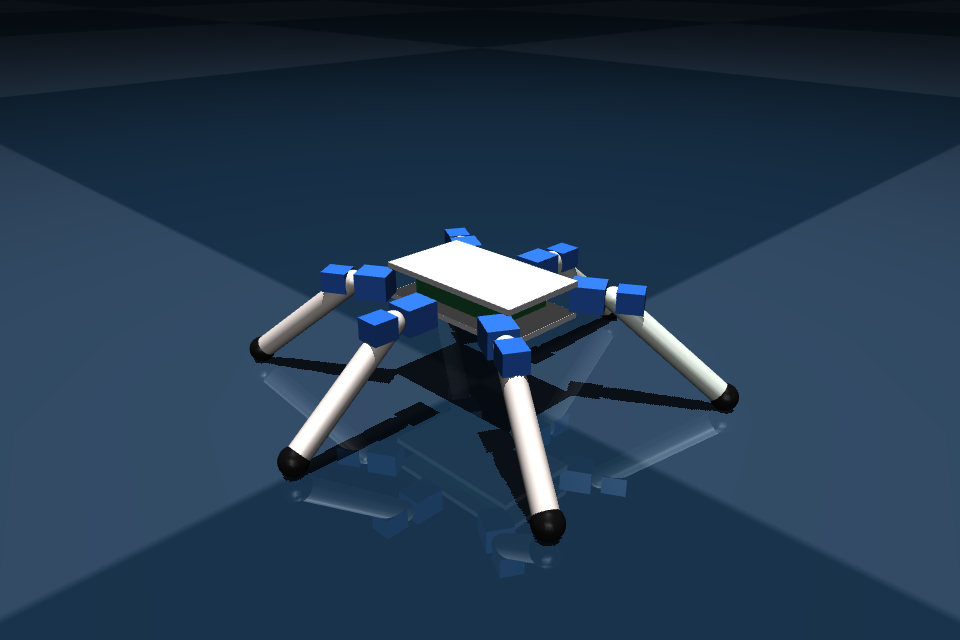
\includegraphics[width=0.92\linewidth]{mujoco_hexapod_sim.png}
  \caption{MuJoCo screenshot of the Walter hexapod model used for PPO training and evaluation (post-settle, zero control; offscreen render).}
  \label{fig:mujoco}
\end{figure}

Figure~\ref{fig:mujoco} confirms the asset geometry and contact setup used for learning; it is a passive settle, not evidence of policy quality. Training and evaluation videos for specific checkpoints provide the appropriate visual readout of learned behavior.

\subsection{MuJoCo PPO evaluations (released checkpoints)}
Table~\ref{tab:rl-eval} quotes short evaluation protocols documented under \url{e90_repo/released_checkpoints/evaluations/}. Rewards are \textbf{not} comparable across configs (different shaping and scaling); forward displacement and path length provide a common physical readout within each experiment family.

\begin{table}[htbp]
  \centering
  \caption{Representative PPO evaluation means (300 env steps per episode unless noted; see each REPORT.md).}
  \label{tab:rl-eval}
  \footnotesize
  \setlength{\tabcolsep}{5pt}
  \renewcommand{\arraystretch}{1.15}
  \begin{tabularx}{\linewidth}{@{}>{\raggedright\arraybackslash}p{2.35cm} >{\raggedright\arraybackslash}X >{\raggedright\arraybackslash}p{1.35cm} >{\raggedright\arraybackslash}p{1.35cm} >{\raggedright\arraybackslash}X@{}}
    \toprule
    Checkpoint & Task / policy & Fwd.\,$+x$ & 2D path & Notes \\
    \midrule
    \url{mlp_clean_run005_best} & Circle path; MLP $256\!\times\!256$ PPO; training run \texttt{mlp\_run\_005} (301k steps). & 0.18\,m & 0.27\,m & Mean reward $\approx 6800$. \\
    \url{terrain_low_shake_run001_best} & Flat, rough, and step terrain; MLP PPO. & 0.33\,m (3 ep.\ mean) & --- & Flat/rough $\approx 0.47$\,m forward; steps harder. \\
    \bottomrule
  \end{tabularx}
\end{table}
\normalsize

\textbf{Reading Table~\ref{tab:rl-eval}.} The rows are \textbf{not} comparable by raw reward (shaping and scaling differ). Forward displacement and path length are coarse physical readouts: the circle-path MLP run shows modest net forward motion and path length consistent with a curved task; the terrain run averages shorter forward progress when steps and roughness dominate. These figures support the claim that \textbf{policies were trained and evaluated in MuJoCo}, not that a single ``best'' locomotion score was achieved across tasks. Treat simulation displacements as \textbf{indicative}, not predictive of hardware distance without deployment tests.

The \texttt{pd\_velocity\_window\_run018\_best} checkpoint is an sCPG + PD + velocity-window experiment with small net displacement in its released short eval---useful as an archival structured-policy datapoint, not a headline locomotion result (see that folder's \texttt{REPORT.md}).

\section{Discussion}

\textbf{What this capstone demonstrates.} The team built a \textbf{named hexapod platform} with documented mechanics, electronics, and cost; implemented an \textbf{optimization-to-firmware} path with reproducible parameters; and ran a \textbf{MuJoCo PPO training and evaluation} workflow with archived checkpoints and configs. Together, that is a credible \textbf{platform-and-methods} outcome: reusable hardware, a defensible open-loop pipeline, and simulation evidence for learned locomotion behaviors under stated rewards.

\textbf{Why full adaptive locomotion is not claimed.} Closing adaptive loops on hardware requires time for IMU bring-up, reflex tuning, safety testing, and power-aware deployment. The phased firmware requirements in \texttt{PHASES.md} were \textbf{not} met in the repository snapshot (Table~\ref{tab:req}); stating that once in requirements and here avoids repeating it in every technical subsection.

\textbf{Technical bottlenecks.} Surrogate versus MuJoCo versus hardware disagree on contact, friction, and servo dynamics; manual degree-to-pulse mapping separates optimized angles from reliable motion; open-loop gaits do not reject disturbances. RL rewards are task-specific, so \textbf{cross-comparing raw returns} across YAML files is misleading---compare displacements and behaviors within a task family only, with humility about sim-to-real.

\textbf{Sim claims.} MuJoCo results show that policies \emph{can} be trained and evaluated under the project's models and rewards. They are \textbf{not} automatic predictors of field performance without transfer experiments.

\textbf{Credible next steps.} Harden IMU read paths and logging on the Teensy; pick one PPO checkpoint and measure a short hardware rollout with matched observation rate; then iterate reflexes or residuals before adding vision or distance-only objectives.

\textbf{Advice for future teams.} Lock a baseline gait and logging format before layering sensors; budget bench time after every simulation milestone; track PCB revisions and BOM multiples from week one.

\section{Conclusion}

This capstone \textbf{established} \emph{Walter}: a twelve-DOF hexapod with CAD/3D-printed structure, custom PCBs, and purchased electronics totaling US\$792.67 in tracked spending. The team \textbf{completed} an open-loop gait optimization loop with deterministic export to firmware, and \textbf{completed} a MuJoCo PPO training and evaluation toolchain with stored checkpoints and representative evaluations. A \textbf{bio-inspired, layered adaptive} control story informed design and simulation choices but was \textbf{not} fully realized on the MCU; that gap is documented in requirements traceability (Table~\ref{tab:req}) rather than hidden. The project provides a \textbf{strong base} for future adaptive and sim-to-real work; code and this report are maintained at \url{https://github.com/HowardWHSrun/WALTER}.

\section*{Acknowledgements}
We thank our advisor, Allan Moser, for guidance on the project. We thank Swarthmore Engineering and shop or lab staff who supported fabrication and testing. No funding sources beyond the Engineering department are declared for this accounting.

\bibliographystyle{ieeetr}
\bibliography{references}

\appendix
\section{Public repository}
\label{app:github}
The public project URL is \url{https://github.com/HowardWHSrun/WALTER}. Appendix paths below refer to the local Engineering~90 workspace layout at the time of writing; the GitHub repository is intended to subsume or mirror these components for reproducibility.

\section{Repository map (selected local paths)}
\begin{itemize}
  \item \textbf{Adaptive firmware and docs:} \texttt{RL Temp/adaptive\_ondevice\_hexapod/README.md}, \texttt{docs/DESIGN.md}, \texttt{docs/ARCHITECTURE.md}, \texttt{docs/PHASES.md}, \texttt{docs/FIRMWARE.md}
  \item \textbf{Firmware sketches:} \texttt{firmware/hexapod\_walking\_v2/}, \texttt{firmware/hexapod\_openloop\_sine/}, \texttt{firmware/set\_zero/}, side-only tests
  \item \textbf{Reduced-order optimization:} \texttt{hexapod\_brain\_roadmap copy/ode\_optimization\_no\_imu/}
  \item \textbf{MuJoCo PPO training:} \texttt{RL Temp/hexapod\_training\_new/} (\texttt{train.py}, \texttt{configs/}, \texttt{runs/})
  \item \textbf{Released checkpoints and evals:} \texttt{RL Temp/e90\_repo/released\_checkpoints/}
  \item \textbf{Presentation notes:} \texttt{Presentation/E90\_MidSemester\_SpeakerScript.tex} (and PDF)
  \item \textbf{This folder (figures):} \texttt{walter\_assembly.png}, \texttt{Body.png}, \texttt{Legs.png}, \texttt{Linkage.png}, \texttt{pcb\_board.png}, \texttt{pcb\_schematic.png}, \texttt{mujoco\_hexapod\_sim.png} (plus originals with longer filenames)
\end{itemize}

\end{document}
